\documentclass[cs4size,a4paper]{ctexart}
\usepackage{caption}



%==================== 数学符号公式 ============
\usepackage{amsmath}                 % AMS LaTeX宏包
\usepackage[style=1]{mdframed}
\usepackage{amsthm}
\usepackage{amsfonts}
\usepackage{mathrsfs}                % 英文花体字 体
\usepackage{bm}                      % 数学公式中的黑斜体
\usepackage{bbding,manfnt}           % 一些图标,如 \dbend
\usepackage{lettrine}                % 首字下沉,命令\lettrine
\def\attention{\lettrine[lines=2,lraise=0,nindent=0em]{\large\textdbend\hspace{1mm}}{}}
\usepackage{longtable}
\usepackage[toc,page]{appendix}
\usepackage{geometry}                % 页边距调整
\usepackage{float}
\geometry{top=3.0cm,bottom=2.7cm,left=2.5cm,right=2.5cm}
\makeatletter
\newcommand{\rmnum}[1]{\romannumeral #1}
\newcommand{\Rmnum}[1]{\expandafter\@slowromancap\romannumeral #1@}
\makeatother
%====================公式按章编号==========================
\numberwithin{equation}{section}
\numberwithin{table}{section}
\numberwithin{figure}{section}
%================= 基本格式预置 ===========================
\usepackage{fancyhdr}
\pagestyle{fancy}
\fancyhf{}
\fancyhead[C]{\zihao{5}  \kaishu 类FTP服务器的实现}
\fancyfoot[C]{~\zihao{5} \thepage~}
\renewcommand{\headrulewidth}{0.65pt}
\CTEXsetup[format={\centering\bfseries\zihao{-2}},name={第, 章}]{section}
\CTEXsetup[nameformat={\bfseries\zihao{3}}]{subsection}
\CTEXsetup[nameformat={\bfseries\zihao{4}}]{subsubsection}
%================== 图形支持宏包 =========================
\usepackage{subfigure}
\usepackage{graphicx}                % 嵌入png图像
\usepackage{color,xcolor}            % 支持彩色文本、底色、文本框等
\usepackage{hyperref}                % 交叉引用
\usepackage{caption}
\captionsetup{figurewithin=section}
%==================== 源码和流程图 =====================
\usepackage{listings}                % 粘贴源代码
\usepackage{xcolor}
\usepackage{color}
\definecolor{dkgreen}{rgb}{0,0.6,0}
\definecolor{gray}{rgb}{0.5,0.5,0.5}
\definecolor{mauve}{rgb}{0.58,0,0.82}
 \usepackage{xcolor}
 \lstset{
  %行号
   basicstyle=\footnotesize,
    numbers=left,
    %背景框
    framexleftmargin=8mm,
    frame=none,
     %背景色
    %backgroundcolor=\color[rgb]{1,1,0.76},
     backgroundcolor=\color[RGB]{245,245,244},
     %样式
   keywordstyle=\bf\color{blue},
   identifierstyle=\bf,
    numberstyle=\color[RGB]{0,192,192},
    commentstyle=\it\color[RGB]{0,96,96},
   stringstyle=\rmfamily\slshape\color[RGB]{128,0,0},
   %显示空格
    showstringspaces=false
 }


%--------------------
\hypersetup{hidelinks}
\usepackage{booktabs}
\usepackage{shorttoc}
\usepackage{tabu,tikz}
\usepackage{float}

\usepackage{multirow}



\tabcolsep=1ex
\tabulinesep=\tabcolsep
\newlength\tikzboxwidth
\newlength\tikzboxheight
\newcommand\tikzbox[1]{%
        \settowidth\tikzboxwidth{#1}%
        \settoheight\tikzboxheight{#1}%
        \begin{tikzpicture}
        \path[use as bounding box]
                (-0.5\tikzboxwidth,-0.5\tikzboxheight)rectangle
                (0.5\tikzboxwidth,0.5\tikzboxheight);
        \node[inner sep=\tabcolsep+0.5\arrayrulewidth,line width=0.5mm,draw=black]
                at(0,0){#1};
        \end{tikzpicture}%
        }

\makeatletter
\def\hlinew#1{%
  \noalign{\ifnum0=`}\fi\hrule \@height #1 \futurelet
   \reserved@a\@xhline}

\newcommand{\tabincell}[2]{\begin{tabular}{@{}#1@{}}#2\end{tabular}}%

\usepackage{subfigure}

\usepackage{CJK}
\usepackage{ifthen}


\usepackage{graphicx}
\newcommand{\HRule}{\rule{\linewidth}{0.5mm}}

\newtheorem{Theorem}{定理}
\newtheorem{Lemma}{引理}
%%使得公式随章节自动编号
\makeatletter
\@addtoreset{equation}{section}
\makeatother
\renewcommand{\theequation}{\arabic{section}.\arabic{equation}}

%-------------------------
	
\usepackage{pythonhighlight}
\usepackage{tikz}
\usepackage{tikz-3dplot}
\usetikzlibrary{shapes,arrows,positioning}
%===================   正文开始    ===================
\begin{document}
\bibliographystyle{gbt7714-2005}     %论文引用格式
%===================  定理类环境定义 ===================
\newtheorem{example}{例}              % 整体编号
\newtheorem{algorithm}{算法}
\newtheorem{theorem}{定理}            % 按 section 编号
\newtheorem{definition}{定义}
\newtheorem{axiom}{公理}
\newtheorem{property}{性质}
\newtheorem{proposition}{命题}
\newtheorem{lemma}{引理}
\newtheorem{corollary}{推论}
\newtheorem{remark}{注解}
\newtheorem{condition}{条件}
\newtheorem{conclusion}{结论}
\newtheorem{assumption}{假设}
%==================重定义 ===================
\renewcommand{\contentsname}{目录}
\renewcommand{\abstractname}{问题的引入}
\renewcommand{\refname}{参考文献}
\renewcommand{\indexname}{索引}
\renewcommand{\figurename}{图}
\renewcommand{\tablename}{表}
\renewcommand{\appendixname}{附录}
\renewcommand{\proofname}{证明}
\renewcommand{\algorithm}{算法}
%============== 封皮和前言 =================
\begin{titlepage}

\begin{center}


% Upper part of the page

\includegraphics[width=0.8\textwidth]{figure/logoNankai}\\[1cm]

\textsc{\LARGE 计算机网络}\\[1.5cm]

\textsc{\LARGE 实验报告}\\[0.5cm]


% Title
\HRule \\[0.4cm]
{ \huge \bfseries 类FTP服务器的实现}\\[0.4cm]

\HRule \\[1.5cm]

% Author and major
\begin{minipage}{0.4\textwidth}
\begin{flushleft} \large
\emph{作者: }
 \textsc{李寅昊}
\end{flushleft}
\end{minipage}
\\
\begin{minipage}{0.4\textwidth}
\begin{flushleft} \large
\emph{学号: }
 \textsc{1611303}
\end{flushleft}
\end{minipage}
\\
\begin{minipage}{0.4\textwidth}
\begin{flushleft} \large
\emph{专业: }
 \textsc{计算机科学与技术}
\end{flushleft}
\end{minipage}

\vfill

% Bottom of the page


\end{center}

\end{titlepage}




\pagestyle{plain}
\pagenumbering{Roman}
%============== 摘要 ======================
\section*{\zihao{3} \centering 实验要求}
\vskip1.0cm

实现一个类FTP功能的协议,实现文件的上传和下载和服务器共享目录的查看。

要求:
\begin{flushleft}

\rmnum{1})下层使用UDP服务。\\

\rmnum{2})支持多用户。\\

\rmnum{3})多用户文件的上传和下载可以仅支持当前目录。\\

\rmnum{4})给出协议的具体内容。(5)给出收发双方的交互日志。\\

\rmnum{5})使用c系列语言进行实现。\\
\end{flushleft}
\clearpage





\pagestyle{empty}
\tableofcontents
\thispagestyle{empty}


%============== 论文正文   =================
\pagestyle{fancy}
\pagenumbering{arabic}
\section{协议内容声明}

\subsection{自定消息类型}
在本程序中,我们自定消息类型,并将其作为客户端和服务器之间交互信息的载体。我们所定消息的定义如下:

\begin{figure}[H]
  \centering
  % Requires \usepackage{graphicx}
  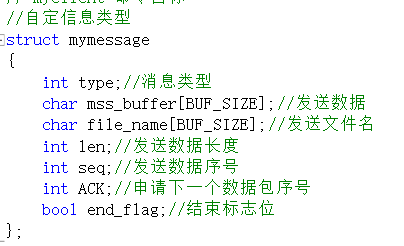
\includegraphics[width=0.8\linewidth]{figure/mymessage}\\
  \caption{mymessage}
\end{figure}

此结构体定义分别被写在myclient类中以及myserver中,从而保证两端信息定义的一致性。在mymessage中,我们分别存放了数据信息,用来发送数据,以及一些必要的标记信息,用来客户端与服务器的交互。
\subsection{自定协议交互过程}

在本次实验中,我们使用一下宏定义信息作为mymessage的type位,用来标记发送信息的类型
\begin{figure}[H]
  \centering
  % Requires \usepackage{graphicx}
  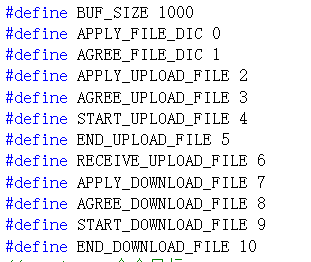
\includegraphics[width=0.8\linewidth]{figure/type}\\
  \caption{mymessage的type位信息}
\end{figure}

协议交互过程如下:

\begin{flushleft}
1)当用户点击获取共享目录时,客户端则会向服务器端发送一个type为APPLY\_FILE\_DIC的消息,服务器端收到此消息后则会回复一个type为AGREE\_FILE\_DIC的消息,并将服务器端的共享目录下的文件加载到发送信息中。\\

2)当用户在客户端选择好要上传的文件并点击开始上传之后,客户端便向服务器发送一条type为APPLY\_UPLOAD\_FILE的消息,并将要上传的文件名包含在消息中。服务器端收到此消息后,便在共享目录创建一个对应的文件,然后发送一条type为AGREE\_UPLOAD\_FILE的消息给客户端。然后客户端逐包发送带有seq的消息,并将type设置为START\_UPLOAD\_FILE。服务器端收到后将收到的包的数据写入创建好的文件,并发送带ACK的消息,将type设置为AGREE\_UPLOAD\_FILE。在客户端发送到最后一个数据包时,会将该条消息的结束标志位end\_flag设置为true。服务器端收到这条消息后将创建的文件流关闭,并向客户端回复一条type为END\_UPLOAD\_FILE的消息,客户端收到后,则跳出。\\


3)当用户在共享目录中选择好要下载的文件,并点击开始下载按钮后,客户端便向服务器端发送一条tpye为APPLY\_DOWNLOAD\_FILE的消息,在这条消息中同样包含了要下载文件的文件名。当服务器端收到这条消息后,则使用文件流打开客户端想要下载的文件,并给客户端打开相应的文件流,回复一条type为AGREE\_DOWNLOAD\_FILE的消息,并把此消息的seq置为-1。而当客户端收到type 未AGREE\_DOWNLOAD\_FILE的消息后,客户端便开始下载工作。每次发送一条type为START\_DOWNLOAD\_FILE的消息给服务器端,客户端收到后回复相应的数据包,客户端收到后将其写入打开的文件流,最后结束后将文件流关闭(此过程与上传过程基本一致)。



\end{flushleft}

\clearpage































\section{协议的具体实现}
\subsection{客户端代码实现}

\subsubsection{总体框架}
我们在窗口类初始化的时候调用另一个封装好的类myclient,用来绑定端口以及处理交互。在窗口类中主要负责实现点击按钮的具体功能以及调用线程持续监听消息。而在myclient 中负责处理接收消息后的处理,以及根据接收到的消息发送对应的信息。
\subsubsection{多线程机制}
我们在窗口类初始化的时候即调用另一个线程,在另一个线程中调用handleReceive函数,使得myclient能够持续接收到消息。

\begin{figure}[H]
  \centering
  % Requires \usepackage{graphicx}
  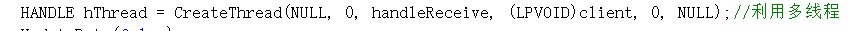
\includegraphics[width=0.8\linewidth]{figure/multiposix}\\
  \caption{多线程}
\end{figure}

相应代码如下:

\begin{flushleft}
\begin{lstlisting}[language={C++},basicstyle=\footnotesize]
//线程调用函数
DWORD WINAPI CClientDlg::handleReceive(LPVOID lpParameter)
{
	myclient* t = (myclient*)lpParameter;
	CString log;
	while(1)
	{
		log.Empty();
		t->handleInteraction();
		CClientDlg* dlg=(CClientDlg*)AfxGetApp()->GetMainWnd(); //获取主窗口
		dlg->m_log+=log;
		dlg->GetDlgItem(IDC_LOG)->SetWindowTextW(dlg->m_log);
	}
	return (DWORD)NULL;
}
\end{lstlisting}
\end{flushleft}

\subsubsection{按钮处理函数}
当用户按下获取文件目录按钮时,客户端向服务器发送type为APPLY\_FILE\_DIC的消息,并且在log中显示对应信息,代码如下:


\begin{flushleft}
\begin{lstlisting}[language={C++},basicstyle=\footnotesize]
//点击获取共享目录按钮
void CClientDlg::OnBnClickedFileDic()
{
	mymessage send_mss;
	send_mss.type = 0;
	//sendto(c_socket,(char*)&temp,sizeof(message),0,(SOCKADDR*)&addrFrom,len);
	sendto(client->c_socket,(char*)&send_mss,sizeof(mymessage),
    0,(SOCKADDR*)&servAddr,sizeof(SOCKADDR));
	CClientDlg* dlg=(CClientDlg*)AfxGetApp()->GetMainWnd(); //获取主窗口
	dlg->m_log += L"开始交互\r\n";
	dlg->m_log+=L"发送查看共享目录请求\r\n";
	dlg->GetDlgItem(IDC_LOG)->SetWindowTextW(dlg->m_log);
	// TODO: 在此添加控件通知处理程序代码
}
\end{lstlisting}
\end{flushleft}

点击开始上传按钮时,客户端用文件流打开相应文件,客户端便向服务器发送一条type为APPLY\_UPLOAD\_FILE的消息,并将要上传的文件名包含在消息中。并向log中显示对应消息。代码如下:

\begin{flushleft}
\begin{lstlisting}[language={C++},basicstyle=\footnotesize]
//点击开始上传按钮
void CClientDlg::OnBnClickedStartUpload()
{
	CClientDlg* dlg=(CClientDlg*)AfxGetApp()->GetMainWnd(); //获取主窗口
	dlg->m_log += L"开始交互\r\n";
	dlg->m_log+=L"发送上传文件命令\r\n";
	dlg->GetDlgItem(IDC_LOG)->SetWindowTextW(dlg->m_log);
	//用文件流打开所选择的文件
	CString upload_file = dlg->m_upload;
	CStringA file_stra(upload_file.GetBuffer(0));
	upload_file.ReleaseBuffer();
	string s = file_stra.GetBuffer(0);
	const char* file_con = s.c_str();
	if (!(client->u_file = fopen(file_con, "rb")))
	{
		AfxMessageBox(_T("创建本地文件失败!"));
	}
	mymessage send_mss;
	int j = 0;
	for(int i = 0;i<upload_file.GetLength();i++)//获取文件名
	{
		if(upload_file[i] == '\\')
		{
			j = 0;
		}
		send_mss.file_name[j] = upload_file[i];
		j++;
	}
	send_mss.file_name[j] = 0;
	//设置消息类型为申请上传文件
	send_mss.type = APPLY_UPLOAD_FILE;
	send_mss.seq = 0;
	sendto(client->c_socket,(char*)
    &send_mss,sizeof(mymessage),0,(SOCKADDR*)&servAddr,sizeof(SOCKADDR));
	if(dlg->m_upload.GetLength()==0)//如果文件选择栏为空,则弹出对话框
	{
		MessageBox(_T("上传文件为空!"));
	}
	dlg->GetDlgItem(IDC_LOG)->SetWindowTextW(dlg->m_log);
	// TODO: 在此添加控件通知处理程序代码
}
\end{lstlisting}
\end{flushleft}

当用户点击开始下载按钮后,客户端便向服务器端发送一条tpye为APPLY\_DOWNLOAD\_FILE的消息,在这条消息中同样包含了要下载文件的文件名,并且log中显示相应消息,代码如下:

\begin{flushleft}
\begin{lstlisting}[language={C++},basicstyle=\footnotesize]
//点击开始下载按钮
void CClientDlg::OnBnClickedStartDownload()
{
	CClientDlg* dlg=(CClientDlg*)AfxGetApp()->GetMainWnd(); //获取主窗口
	dlg->m_log += L"开始交互\r\n";
	dlg->m_log+=L"发送下载文件命令\r\n";
	mymessage send_mss;
	//设置消息类型为申请下载
	send_mss.type = APPLY_DOWNLOAD_FILE;
	//获取文件名
	for(int i=0;i<m_download.GetLength();i++)
	{
		send_mss.file_name[i] = m_download[i];
	}
	send_mss.file_name[m_download.GetLength()]=0;
	if(dlg->m_download.GetLength()==0)//如果文件选择栏为空,则弹出对话框
	{
		MessageBox(_T("下载文件为空!"));
	}
	char path[MAX_PATH + 1] = { 0 };
	GetModuleFileNameA(NULL, path, MAX_PATH);
	(strrchr(path, '\\'))[0] = 0; // 删除文件名,只获得路径字串
	client->full_ACK = 0;
	strcat(path,"\\");
	client->d_file = fopen(strcat(path,send_mss.file_name),"wb");
	sendto(client->c_socket,(char*)
    &send_mss,sizeof(mymessage),0,(SOCKADDR*)&servAddr,sizeof(SOCKADDR));
	dlg->GetDlgItem(IDC_LOG)->SetWindowTextW(dlg->m_log);
}
\end{lstlisting}
\end{flushleft}


\subsubsection{交互的实现}

当客户端收到type为AGREE\_FILE\_DIC的消息时,客户端便将收到的数据(即共享文件目录)显示在相应窗口中,并在log中添加相应消息。代码如下:

\begin{flushleft}
\begin{lstlisting}[language={C++},basicstyle=\footnotesize]
//服务器同意上传文件
case AGREE_UPLOAD_FILE:
{
	mymessage send_mss;
	//用文件流读文件文件
	int batch_num = fread(send_mss.mss_buffer,1, BUF_SIZE , u_file);
	send_mss.type = START_UPLOAD_FILE;
	int j = 0;
	dlg->m_log += L"上传文件中\r\n";
	CString upload_file = dlg->m_upload;
	send_mss.len = batch_num;
	send_mss.seq = recv.ACK;
	//读出内容长度小于BUF_SIZE,则证明上传完成
	if(batch_num < BUF_SIZE)
	{
		dlg->m_log += L"上传文件完成\r\n";
		send_mss.end_flaaaaaaa[P-=ag = true;
	}
	else
	{
		send_mss.end_flag = false;
	}
	sendto(c_socket,(char*)&send_mss, sizeof(mymessage), 0,
				(SOCKADDR*)&addrFrom, sizeof(SOCKADDR));
	dlg->GetDlgItem(IDC_LOG)->SetWindowTextW(dlg->m_log);
	
	return;
}
\end{lstlisting}
\end{flushleft}


当客户端收到type为AGREE\_UPLOAD\_FILE的消息时,客户端逐包发送带有seq的消息,并将type设置为START\_UPLOAD\_FILE。相应代码如下:

\begin{flushleft}
\begin{lstlisting}[language={C++},basicstyle=\footnotesize]
//服务器同意上传文件
case AGREE_UPLOAD_FILE:
{
	mymessage send_mss;
	//用文件流读文件文件
	int batch_num = fread(send_mss.mss_buffer,1, BUF_SIZE , u_file);
	send_mss.type = START_UPLOAD_FILE;
	int j = 0;
	dlg->m_log += L"上传文件中\r\n";
	CString upload_file = dlg->m_upload;
	send_mss.len = batch_num;
	send_mss.seq = recv.ACK;
	//读出内容长度小于BUF_SIZE,则证明上传完成
	if(batch_num < BUF_SIZE)
	{
		dlg->m_log += L"上传文件完成\r\n";
		send_mss.end_flag = true;
	}
	else
	{
		send_mss.end_flag = false;
	}
	sendto(c_socket,(char*)&send_mss, sizeof(mymessage), 0,
				(SOCKADDR*)&addrFrom, sizeof(SOCKADDR));
	dlg->GetDlgItem(IDC_LOG)->SetWindowTextW(dlg->m_log);
	
	return;
}
\end{lstlisting}
\end{flushleft}

当客户端收到type为END\_UPLOAD\_FILE的消息时,直接跳出。代码如下:
\begin{flushleft}
\begin{lstlisting}[language={C++},basicstyle=\footnotesize]
//上传完成,则跳出
case END_UPLOAD_FILE:
{

	c_posting = false;
	return;
}
\end{lstlisting}
\end{flushleft}


当客户端收到type为AGREE\_DOWNLOAD\_FILE的消息时,客户端便开始下载工作。代码如下:


\begin{flushleft}
\begin{lstlisting}[language={C++},basicstyle=\footnotesize]
//服务器同意下载文件
case AGREE_DOWNLOAD_FILE:
{
	if(recv.seq == -1)
	{
		dlg->m_log += L"开始下载文件\r\n";
	}
	mymessage send_mss;
	send_mss.type = START_DOWNLOAD_FILE;
	//ACK与seq相等,则ACK与len相加后继续发送
	if(full_ACK == recv.seq)
	{
		fwrite(recv.mss_buffer,recv.len,1,d_file);
		dlg->m_log += L"下载文件中\r\n";
		send_mss.type = AGREE_UPLOAD_FILE;
		full_ACK = send_mss.ACK = full_ACK + recv.len;
	}
	else
	{
		send_mss.ACK = full_ACK;
	}
	//结束为为true且不处于开始发送状态,则关闭文件,下载完成
	if(recv.end_flag && recv.seq!=-1)
	{
		fclose(d_file);
		send_mss.type = END_DOWNLOAD_FILE;
		dlg->m_log += L"下载文件完成\r\n";
	}
	else
	{
		send_mss.type = START_DOWNLOAD_FILE;
	}
	sendto(c_socket,(char*)&send_mss,sizeof(mymessage),
    0,(SOCKADDR*)&addrFrom,sizeof(SOCKADDR));
	return;
}
\end{lstlisting}
\end{flushleft}

\subsection{服务器端代码实现}

\subsubsection{总体框架}

在服务器端我们采用同样的框架,在窗口类初始化的时候调用myserver类使其绑定相应端口并处理交互数据。利用与客户端一样的多线程机制使其能够持续监听消息。

\subsubsection{交互的实现}

当服务器端收到type为APPLY\_FILE\_DIC的消息时,之后服务器端查看共享目录的文件列表,将其放在发送报文中,并将其type设置为AGREE\_FILE\_DIC,并将其发送给客户端。代码如下:

\begin{flushleft}
\begin{lstlisting}[language={C++},basicstyle=\footnotesize]
//客户端申请访问共享目录
case APPLY_FILE_DIC:
{
	CServerDlg* dlg=(CServerDlg*)AfxGetApp()->GetMainWnd(); //获取主窗口
	dlg->m_log+=L"收到请求共享目录消息.\r\n";
	send_mss.type = AGREE_FILE_DIC;
	for (int j = 1; j < BUF_SIZE; j++)
	{
		send_mss.mss_buffer[j] = 0;
	}
	char szFilePath[MAX_PATH + 1] = { 0 };
	GetModuleFileNameA(NULL, szFilePath, MAX_PATH);
	(strrchr(szFilePath, '\\'))[0] = 0; // 删除文件名,只获得路径字串
	string p;
	//文件句柄
	long   hFile = 0;
	//文件信息
	struct _finddata_t fileinfo;
	if ((hFile = _findfirst(p.assign(szFilePath)
    .append("\\*").c_str(), &fileinfo)) != -1)
	{
		do
		{
			strncat(send_mss.mss_buffer, 
        strncat(fileinfo.name,"\r\n",5), BUF_SIZE);
		} while (_findnext(hFile, &fileinfo) == 0);
		_findclose(hFile);
	}
	send_mss.mss_buffer[BUF_SIZE-1] = '\n';
	//displayShared(sendBuf);
	sendto(s_socket, (char*)&send_mss, sizeof(mymessage), 
    0,(SOCKADDR*)&clntAddr, sizeof(SOCKADDR));
	end = true;
	dlg->m_log+=L"发送共享文件目录\r\n";
	break;
}
\end{lstlisting}
\end{flushleft}

当服务器端收到type为APPLY\_UPLOAD\_FILE的消息时,客户端便根据发来消息的文件名创建文件,并把回复信息的type设置为AGREE\_UPLOAD\_FILE。代码如下:

\begin{flushleft}
\begin{lstlisting}[language={C++},basicstyle=\footnotesize]
//客户端申请上传文件
case APPLY_UPLOAD_FILE:
{
	CServerDlg* dlg=(CServerDlg*)AfxGetApp()->GetMainWnd(); //获取主窗口
	dlg->m_log+=L"收到请求上传文件消息.\r\n";
	//设置发送信息的类型为AGREE_UPLOAD_FILE
	mymessage send_mss;
	send_mss.type = AGREE_UPLOAD_FILE;
	send_mss.ACK = 0;
	sendto(s_socket, (char*)&send_mss, strLen, 0,
    (SOCKADDR*)&clntAddr, sizeof(SOCKADDR));
	char path[MAX_PATH + 1] = { 0 };
	GetModuleFileNameA(NULL, path, MAX_PATH);
	(strrchr(path, '\\'))[0] = 0; // 删除文件名,只获得路径字串
	full_ACK = 0;
	u_file = fopen(strcat(path,recv_mss.file_name),"wb");
	end = true;
	dlg->m_log+=L"发送同意上传文件消息\r\n";
	break;
}
\end{lstlisting}
\end{flushleft}

当服务器端收到type为START\_UPLOAD\_FILE的消息时,客户端向已创建的文件中写入发送消息包含的文件数据,并根据发过来的seq回复对应的ACK,代码如下:

\begin{flushleft}
\begin{lstlisting}[language={C++},basicstyle=\footnotesize]
//客户端开始上传文件
case START_UPLOAD_FILE:
{
	CServerDlg* dlg=(CServerDlg*)AfxGetApp()->GetMainWnd(); //获取主窗口
	//发送的ACK与初始seq相等,则继续发送
	if(recv_mss.seq == full_ACK)
	{
		fwrite(recv_mss.mss_buffer,recv_mss.len,1,u_file);
		dlg->m_log += L"接收上传文件中\r\n";
		send_mss.type = AGREE_UPLOAD_FILE;
		full_ACK = send_mss.ACK = full_ACK + recv_mss.len;
	}
	//如果不相等,则继续发送上一个ACK
	else
	{
		send_mss.ACK = full_ACK;
	}
	if(recv_mss.end_flag)
	{
		fclose(u_file);
		send_mss.type = END_UPLOAD_FILE;
		dlg->m_log += L"接收上传文件完成\r\n";
	}
	else
	{
		send_mss.type = AGREE_UPLOAD_FILE;
	}
	sendto(s_socket, (char*)&send_mss, 
    sizeof(mymessage), 0,(SOCKADDR*)&clntAddr, sizeof(SOCKADDR));
	end = true;
	break;
}
\end{lstlisting}
\end{flushleft}

当服务器端收到type为APPLY\_DOWNLOAD\_FILE的消息时,打开发送消息所包含的文件名,并将回复信息的type设置为AGREE\_DOWNLOAD\_FILE,代码如下:

\begin{flushleft}
\begin{lstlisting}[language={C++},basicstyle=\footnotesize]
//客户端申请下载文件
case APPLY_DOWNLOAD_FILE:
{
	CServerDlg* dlg=(CServerDlg*)AfxGetApp()->GetMainWnd(); //获取主窗口
	dlg->m_log+=L"收到请求下载文件消息.\r\n";
	mymessage send_mss;
	send_mss.type = AGREE_DOWNLOAD_FILE;
	send_mss.seq = -1;
	sendto(s_socket, (char*)&send_mss, sizeof(mymessage), 
    0,(SOCKADDR*)&clntAddr, sizeof(SOCKADDR));
	dlg->m_log+=L"发送同意下载文件消息.\r\n";
	//dlg->m_log+=CString(recv_mss.mss_buffer);
	char path[MAX_PATH + 1] = { 0 };
	GetModuleFileNameA(NULL, path, MAX_PATH);
	(strrchr(path, '\\'))[0] = 0; // 删除文件名,只获得路径字串
	full_ACK = 0;
	strcat(path,"\\");
	//用文件流打开文件
	d_file = fopen(strcat(path,recv_mss.file_name),"rb");
	end = true;
	break;

}
\end{lstlisting}
\end{flushleft}


当服务器端收到type为START\_DOWNLOAD\_FILE的消息时,服务器读取之前打开的的文件流,并将其放到发送的消息中,并根据ACK发送seq,当读取文件结束时,将结束标志位置1,代码如下:

\begin{flushleft}
\begin{lstlisting}[language={C++},basicstyle=\footnotesize]
//客户端开始下载文件
case START_DOWNLOAD_FILE:
{
	mymessage send_mss;
	int batch_num = fread(send_mss.mss_buffer,1, BUF_SIZE , d_file);
	CServerDlg* dlg=(CServerDlg*)AfxGetApp()->GetMainWnd(); //获取主窗口
	dlg->m_log+=L"开始下载文件.\r\n";
	send_mss.len = batch_num;
	send_mss.seq = recv_mss.ACK;
	//如果文件流读出来的大小小于BUF_SIZE,则证明下载文件完毕,设置结束标志位。
	if(batch_num < BUF_SIZE)
	{
		dlg->m_log += L"下载文件完成\r\n";
		send_mss.end_flag = true;
	}
	else
	{
		send_mss.end_flag = false;
	}
	send_mss.type = AGREE_DOWNLOAD_FILE;
	sendto(s_socket,(char*)&send_mss, sizeof(mymessage), 0,
				(SOCKADDR*)&clntAddr, sizeof(SOCKADDR));
	end = true;
	break;
}
\end{lstlisting}
\end{flushleft}

当服务器端收到type为END\_DOWNLOAD\_FILE的消息时,直接跳出。代码如下:

\begin{flushleft}
\begin{lstlisting}[language={C++},basicstyle=\footnotesize]
//客户端下载结束
case END_DOWNLOAD_FILE:
{
	break;
}
\end{lstlisting}
\end{flushleft}

\subsection{可靠性的保证}

首先我们模仿FTP设置了seq和ACK值只有两者相对应时才能进行传输,从而保证了没有乱序。此外,我们设置了超时重传机制,将超时时间设置为2s,从而超时时,将上一次数据重新发送,代码如下:

\begin{flushleft}
\begin{lstlisting}[language={C++},basicstyle=\footnotesize]
//设置超时重传
int timeout = 2000;      //设置超时时间为2s
setsockopt(s_socket,SOL_SOCKET,SO_RCVTIMEO,(const char*)&timeout,sizeof(int));
recv_mss.type = -1;
\end{lstlisting}
\end{flushleft}

当超时时,上一个要发送的数据则被重新发送。
\clearpage

\section{实验结果展示}
\subsection{客户端和服务器端的初始界面}
运行客户和服务器两个工程,我们便得到了初始界面,如下:
\begin{figure}[H]
  \centering
  % Requires \usepackage{graphicx}
  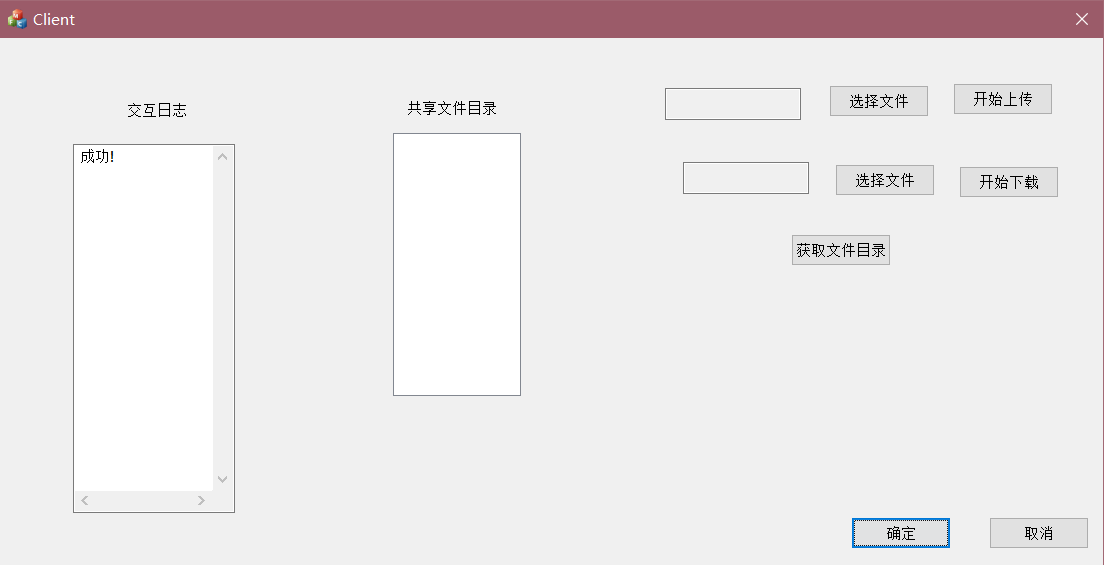
\includegraphics[width=0.8\linewidth]{figure/client_init}\\
  \caption{客户端初始界面}
\end{figure}

\begin{figure}[H]
  \centering
  % Requires \usepackage{graphicx}
  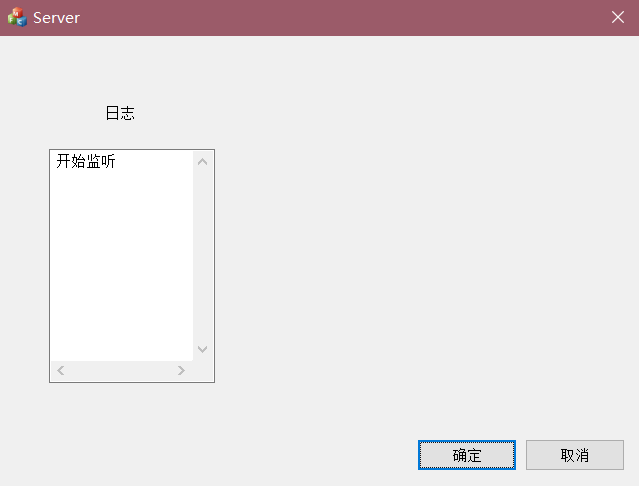
\includegraphics[width=0.8\linewidth]{figure/server_init}\\
  \caption{服务器端端初始界面}
\end{figure}

\subsection{共享目录的获取}
我们在客户端点击获取共享目录按钮,便可以获得服务器端的共享目录,两端变化如下:

\begin{figure}[H]
  \centering
  % Requires \usepackage{graphicx}
  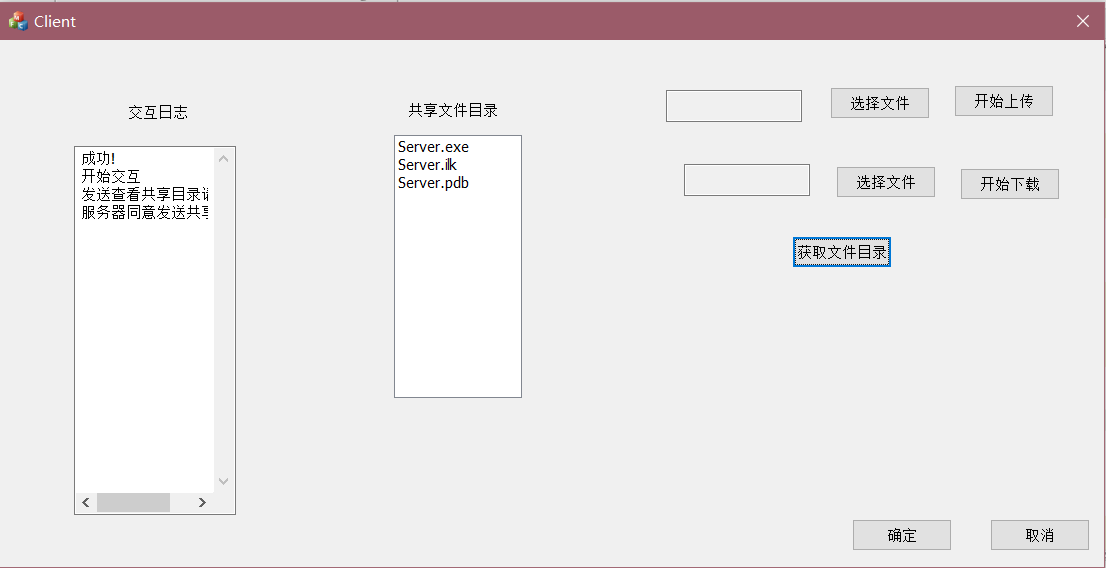
\includegraphics[width=0.8\linewidth]{figure/client_file_dic}\\
  \caption{客户端获取共享目录}
\end{figure}

\begin{figure}[H]
  \centering
  % Requires \usepackage{graphicx}
  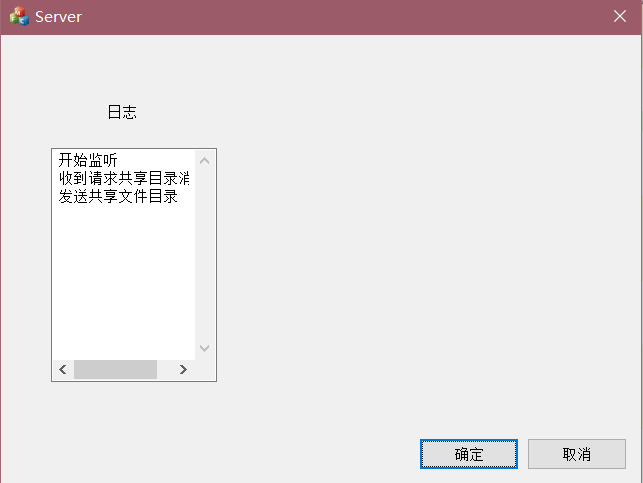
\includegraphics[width=0.8\linewidth]{figure/server_file_dic}\\
  \caption{服务器端获取共享目录}
\end{figure}

\subsection{客户端上传文件}
我们选择上传文件后点击“开始上传”按钮,我们便可以进行文件的上传了
\begin{figure}[H]
  \centering
  % Requires \usepackage{graphicx}
  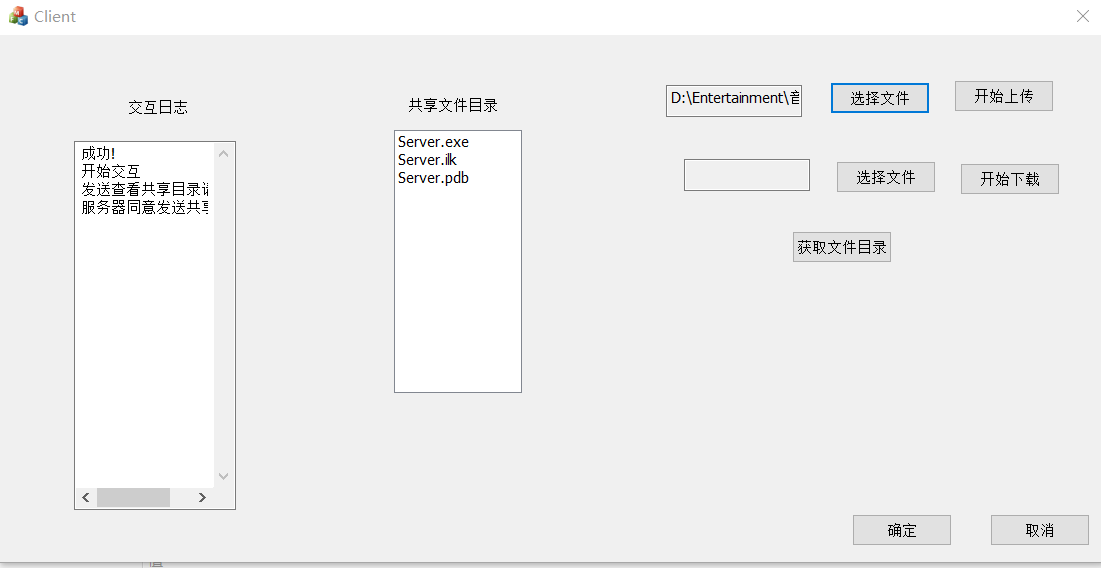
\includegraphics[width=0.8\linewidth]{figure/client_before_upload}\\
  \caption{客户端上传前}
\end{figure}
\begin{figure}[H]
  \centering
  % Requires \usepackage{graphicx}
  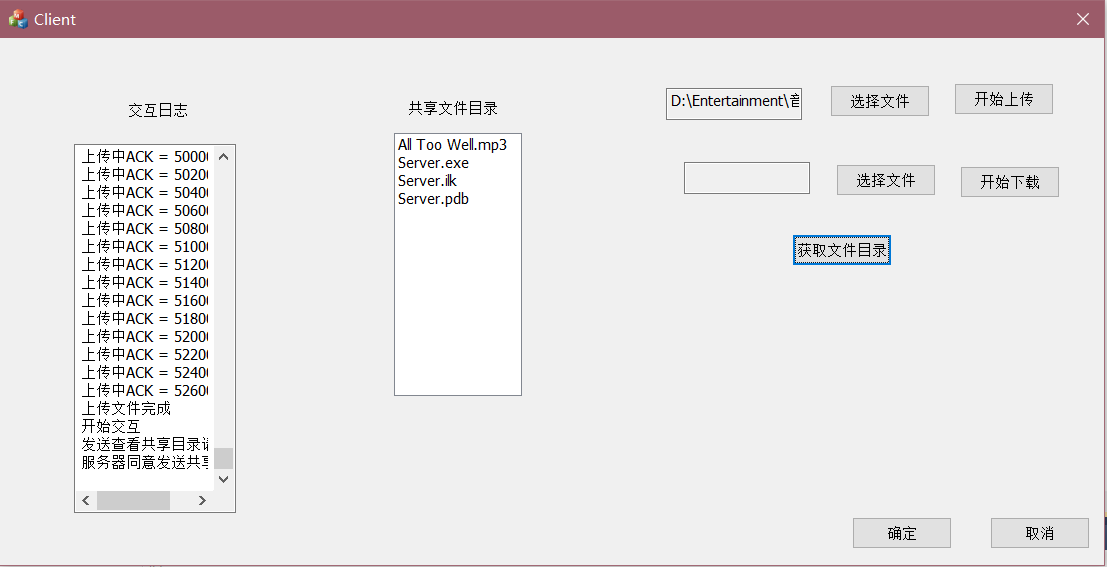
\includegraphics[width=0.8\linewidth]{figure/client_after_upload}\\
  \caption{客户端上传完成}
\end{figure}


\begin{figure}[H]
  \centering
  % Requires \usepackage{graphicx}
  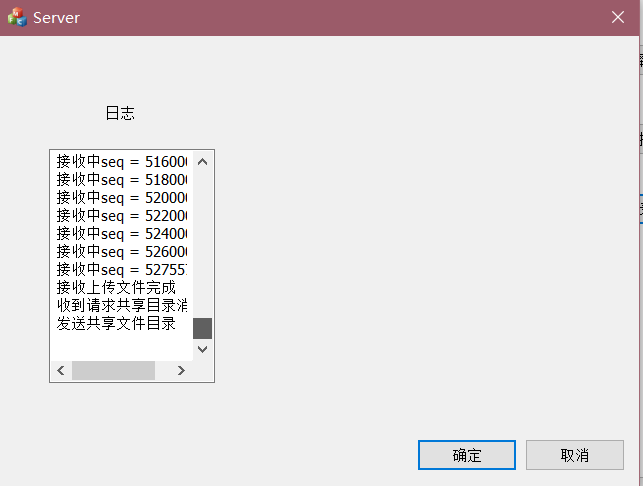
\includegraphics[width=0.8\linewidth]{figure/server_upload}\\
  \caption{服务器端接收上传完成}
\end{figure}
可以看到,共享目录增加了上传的文件,实验成功。

\subsection{客户端下载文件}
我们在客户端的共享目录中选择要下载的文件,然后点击“开始下载”按钮后,我们便可以进行文件的下载了。
\begin{figure}[H]
  \centering
  % Requires \usepackage{graphicx}
  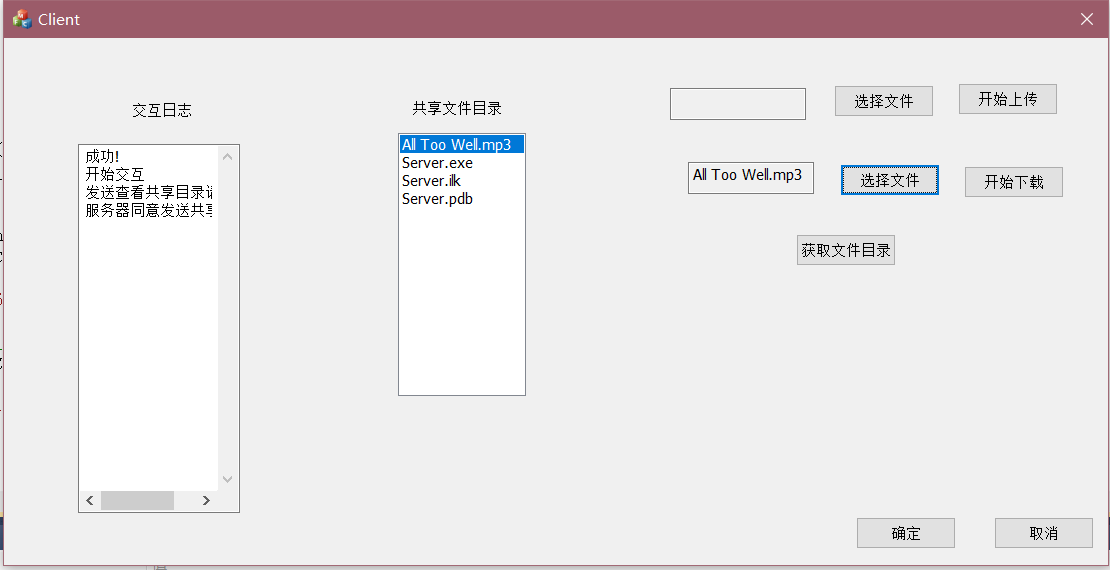
\includegraphics[width=0.8\linewidth]{figure/client_before_download}\\
  \caption{客户端下载前}
\end{figure}
\begin{figure}[H]
  \centering
  % Requires \usepackage{graphicx}
  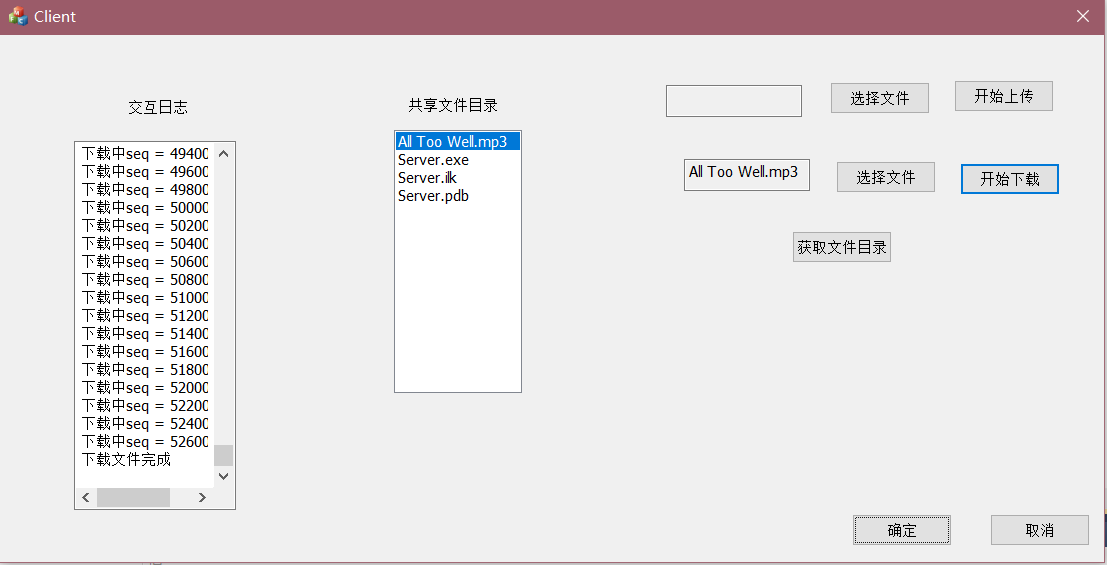
\includegraphics[width=0.8\linewidth]{figure/client_after_download}\\
  \caption{客户端下载完成后}
\end{figure}
\begin{figure}[H]
  \centering
  % Requires \usepackage{graphicx}
  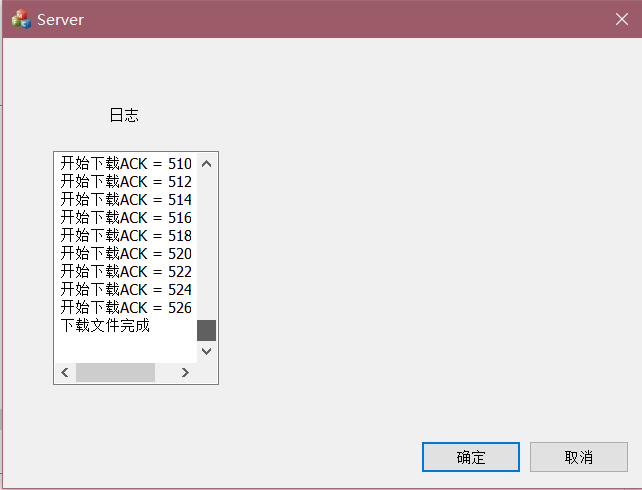
\includegraphics[width=0.8\linewidth]{figure/server_download}\\
  \caption{服务器端下载完成后}
\end{figure}

我们在客户端文件夹中可以看到获取了正确的文件,实验成功。

\subsection{多用户}

\begin{figure}[H]
  \centering
  % Requires \usepackage{graphicx}
  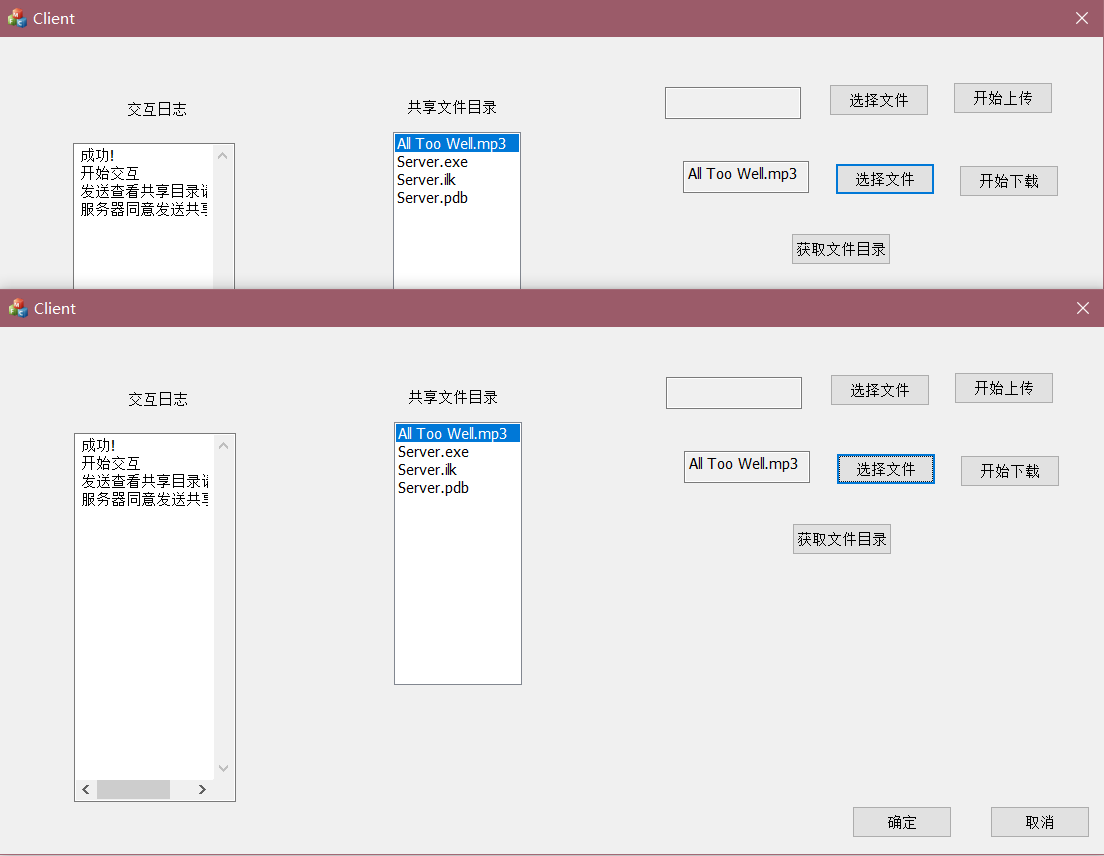
\includegraphics[width=0.8\linewidth]{figure/multiclient_before_download}\\
  \caption{多用户下载前}
\end{figure}
\begin{figure}[H]
  \centering
  % Requires \usepackage{graphicx}
  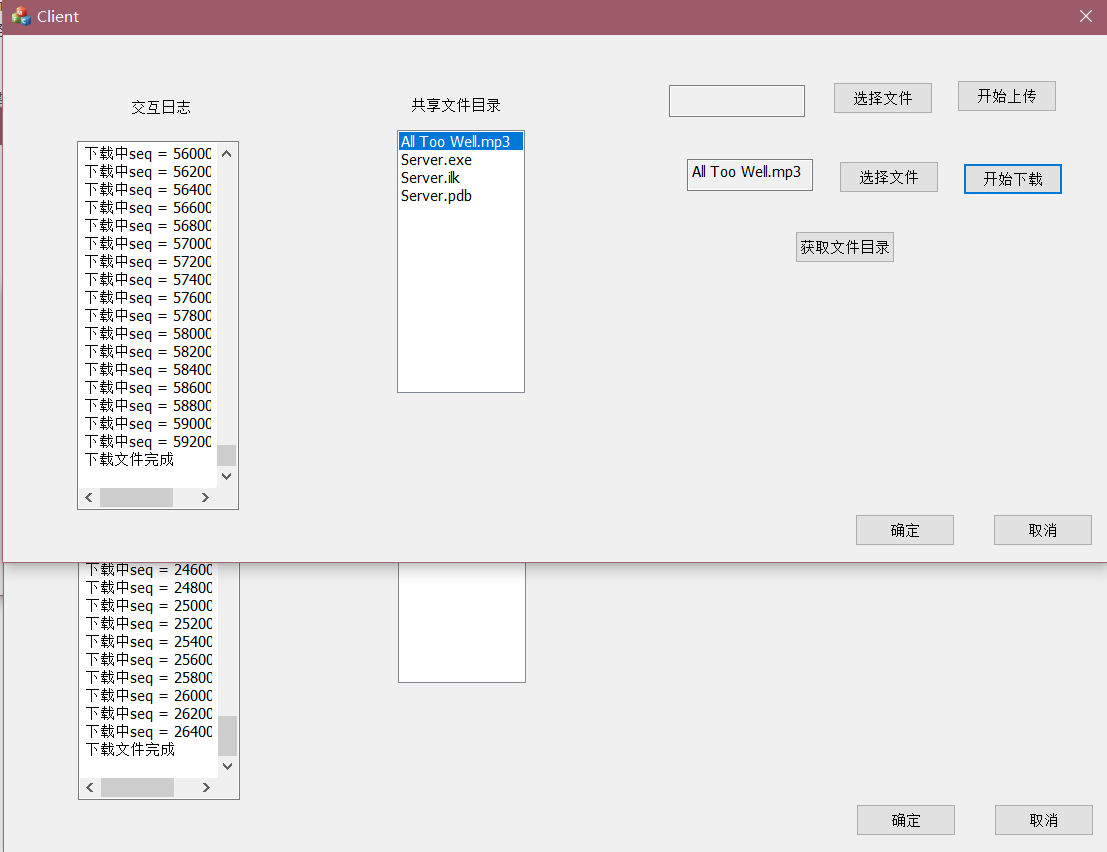
\includegraphics[width=0.8\linewidth]{figure/multiclient_after_download}\\
  \caption{多用户下载完成后}
\end{figure}
\begin{figure}[H]
  \centering
  % Requires \usepackage{graphicx}
  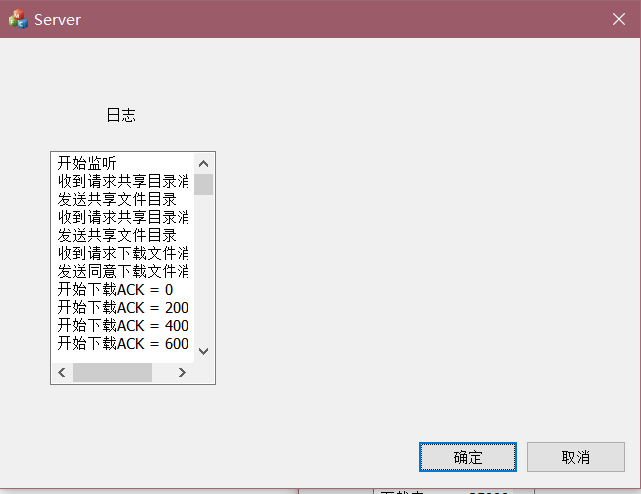
\includegraphics[width=0.8\linewidth]{figure/multiserver_download}\\
  \caption{多用户服务器端下载完成后}
\end{figure}

可以看到在服务器端显示了两条下载完成记录,两个客户端也正确完成了下载。
\clearpage

%============= 参考文献 =====================
%\section*{ \centering 参考文献}
\begin{flushleft}
[1] 位、字、字节的区别 | 汇编伪指令db,dw,dd
[B/OL].http://blog.csdn.net/aurorayqz/article/details/71549166
\par
\vspace{3ex}
[2] MASM32 控制台输入输出
[B/OL].http://blog.csdn.net/xboxmicro/article/details/21658003
\par
\vspace{3ex}
[3] Kip R.Irvine,温玉杰(译),梅广宇(译)等.Intel汇编语言设计(第五版)[M].北京:电子工业出版社,2007
\par
\vspace{3ex}
[4] Jeffrey D.Ullman,Ravi Sethi,Monica S.Lam,Alfred V.Aho.《编译原理》.
机械工业出版社
\end{flushleft}
\addcontentsline{toc}{section}{参考文献}
\clearpage


%\usepackage{cite}
%\bibliographystyle{gbt7714-2005}
%\bibliography{bibfile}%%我们的例子应该是\bibliography{cited}
%\newpage
\appendix %添加附录编号

%%附录第一个章节
\section{附录:C代码}


%%斐波那契
\begin{lstlisting}[language={C}]
//T8255-1.c
//8255并口控制器应用实验  B口输入,A口输出

#include <stdio.h>
#include <stdlib.h>
#include <conio.h>
#include <bios.h>
#include <ctype.h>
#include <process.h>

void key(void);
void delay(int time);

//****************根据查看配置信息修改下列符号值*******************
#define  IOY0         0x3000
//*****************************************************************
#define  MY8255_A     IOY0 + 0x00*2
#define  MY8255_B     IOY0 + 0x01*2
#define  MY8255_C     IOY0 + 0x02*2
#define  MY8255_MODE  IOY0 + 0x03*2

char as[4] = {0x10,0x20,0x40,0x80};

void main()
{
	

	int i = 0;
	while(1)
	{
		for(i = 0;i<4;i++)
		{
            	int a;
	            int b;
	for(a=0;a<=0x10;a++)
	{
		for(b=0;b<=0x7000;b++)
		{
		outp(0x3008, as[i]);
		}
	}
			
		//	delay(0x10);
			key();
		}
	}
		
	

}

void key(void)
{
	if (bioskey(1) != 0)
	{
		exit(0);
	}
}

void delay(int time)
{
	int i;
	int j;
	for(i=0;i<=time;i++)
	{
		for(j=0;j<=0x7000;j++)
		{
		}
	}
	return;
}
\end{lstlisting}

%=============  致谢  ======================





\end{document}
%%%%%%%%%% 结束 %%%%%%%%%%
